\chapter{Implementation}\label{ch:implementation}

%\Todo{Here we can put pictures and codes snippets}\\

%Instead of having a huge amount of different pre-recorded sound files, which need a lot of space, we eliminate the problem to a \colorbox{pink}{2D look up}, where the algorithm matches the object first and then the exact point of the object that collided with some other object.
%

\section{Recordings}\label{sec:recordings}

The measurements were conducted in an anechoic chamber at \gls{DTU}'s Department of Electrical Engineering using a microphone placed one meter away from the struck object. To record the sounds a Bruel \& Kjær's half inch pressure field microphone type 4192 and a microphone preamplifier power supply type 5935L, as well as the 744T digital audio recorder from Sound Devices at 44100 Hz sampling frequency were used. The setup can be seen in figure \ref{fig:experiment}.

\begin{figure}[H]
  \centering
    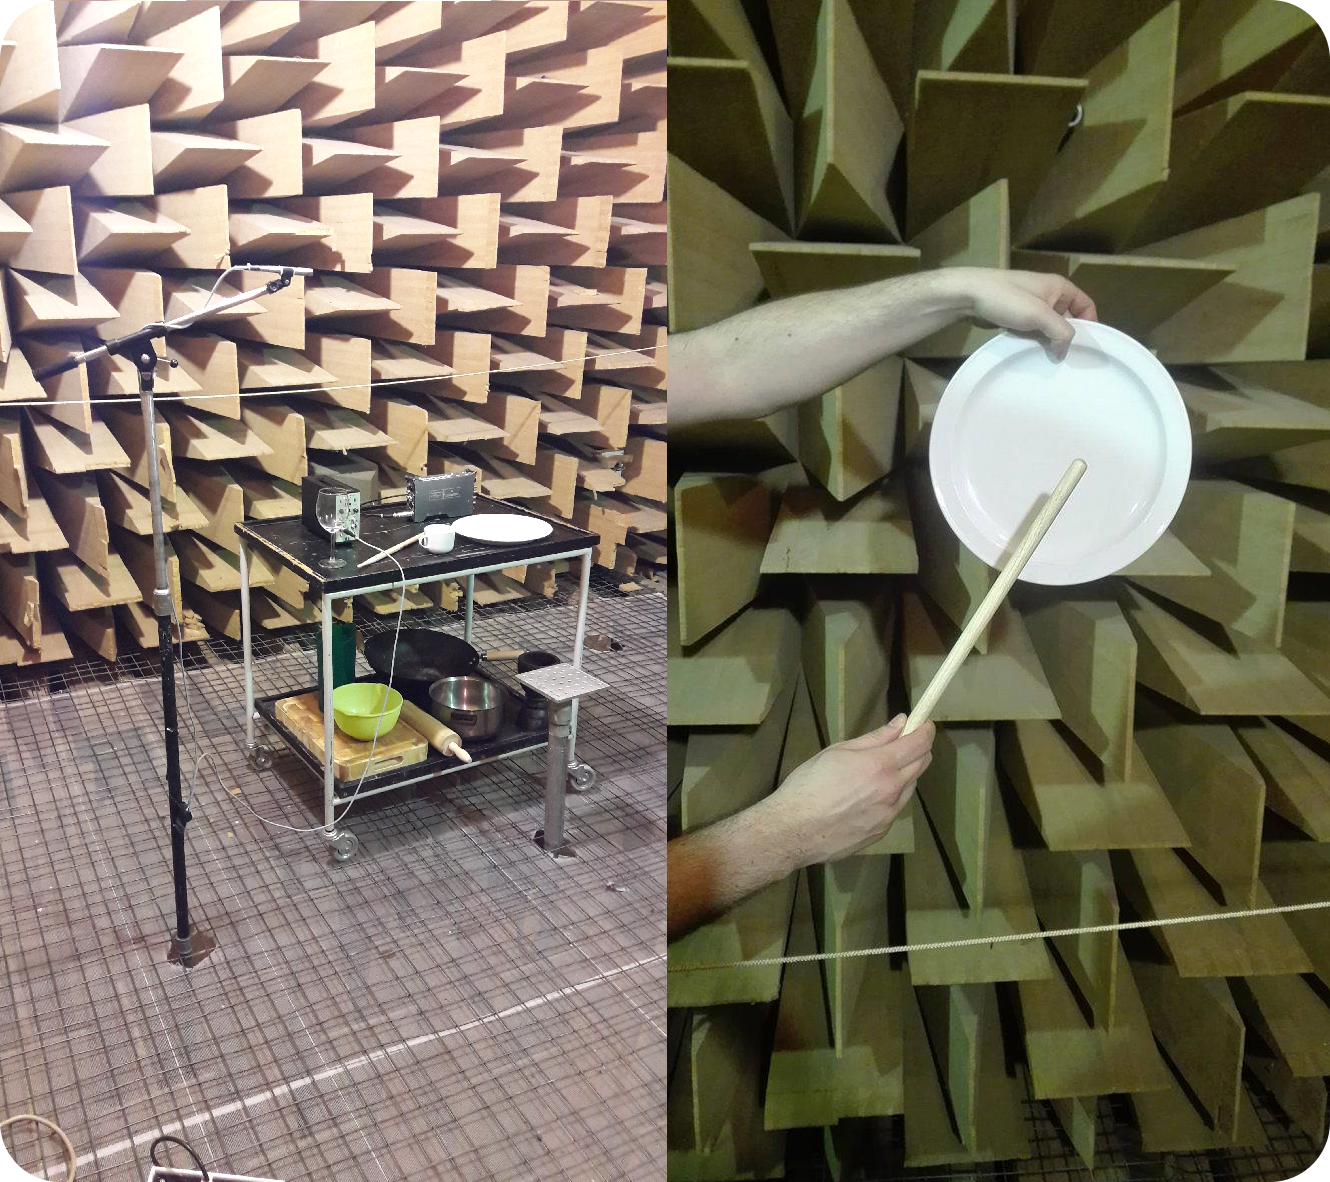
\includegraphics[width=0.7\textwidth]{experimentpic_r.png}
      \caption{Picture of the setup for the measurements (left) and of a struck object (right).}\label{fig:experiment}
\end{figure}

To control the impact, the objects were hit by hand with a wooden drumstick (figure \ref{fig:experiment} (right)) while trying to use the same impulsive force. Prior to the recordings, every object was divided into different surface areas depending on its shape and the sound produced by these areas (see figure \ref{fig:pot_sep} in \ref{sec:discretization}). Therefore, several impact locations were chosen and recorded for every object.

Eleven objects of everyday life made of five different materials (plastic, wood, ceramic, glass and metal) were used for the experiment. The idea of choosing these objects came firstly from the need of owning them (to perform the recording) and our ability to model them for the demo (as they should be simple enough). Secondly, since we wished to test the immersion of the synthesized sounds on users, we wanted to be sure that the sounds used are familiar to them. In figure \ref{fig:objects} both real and modeled objects are shown. 

\begin{figure}[H]
    \centering
    \begin{subfigure}[b]{0.8\textwidth}
        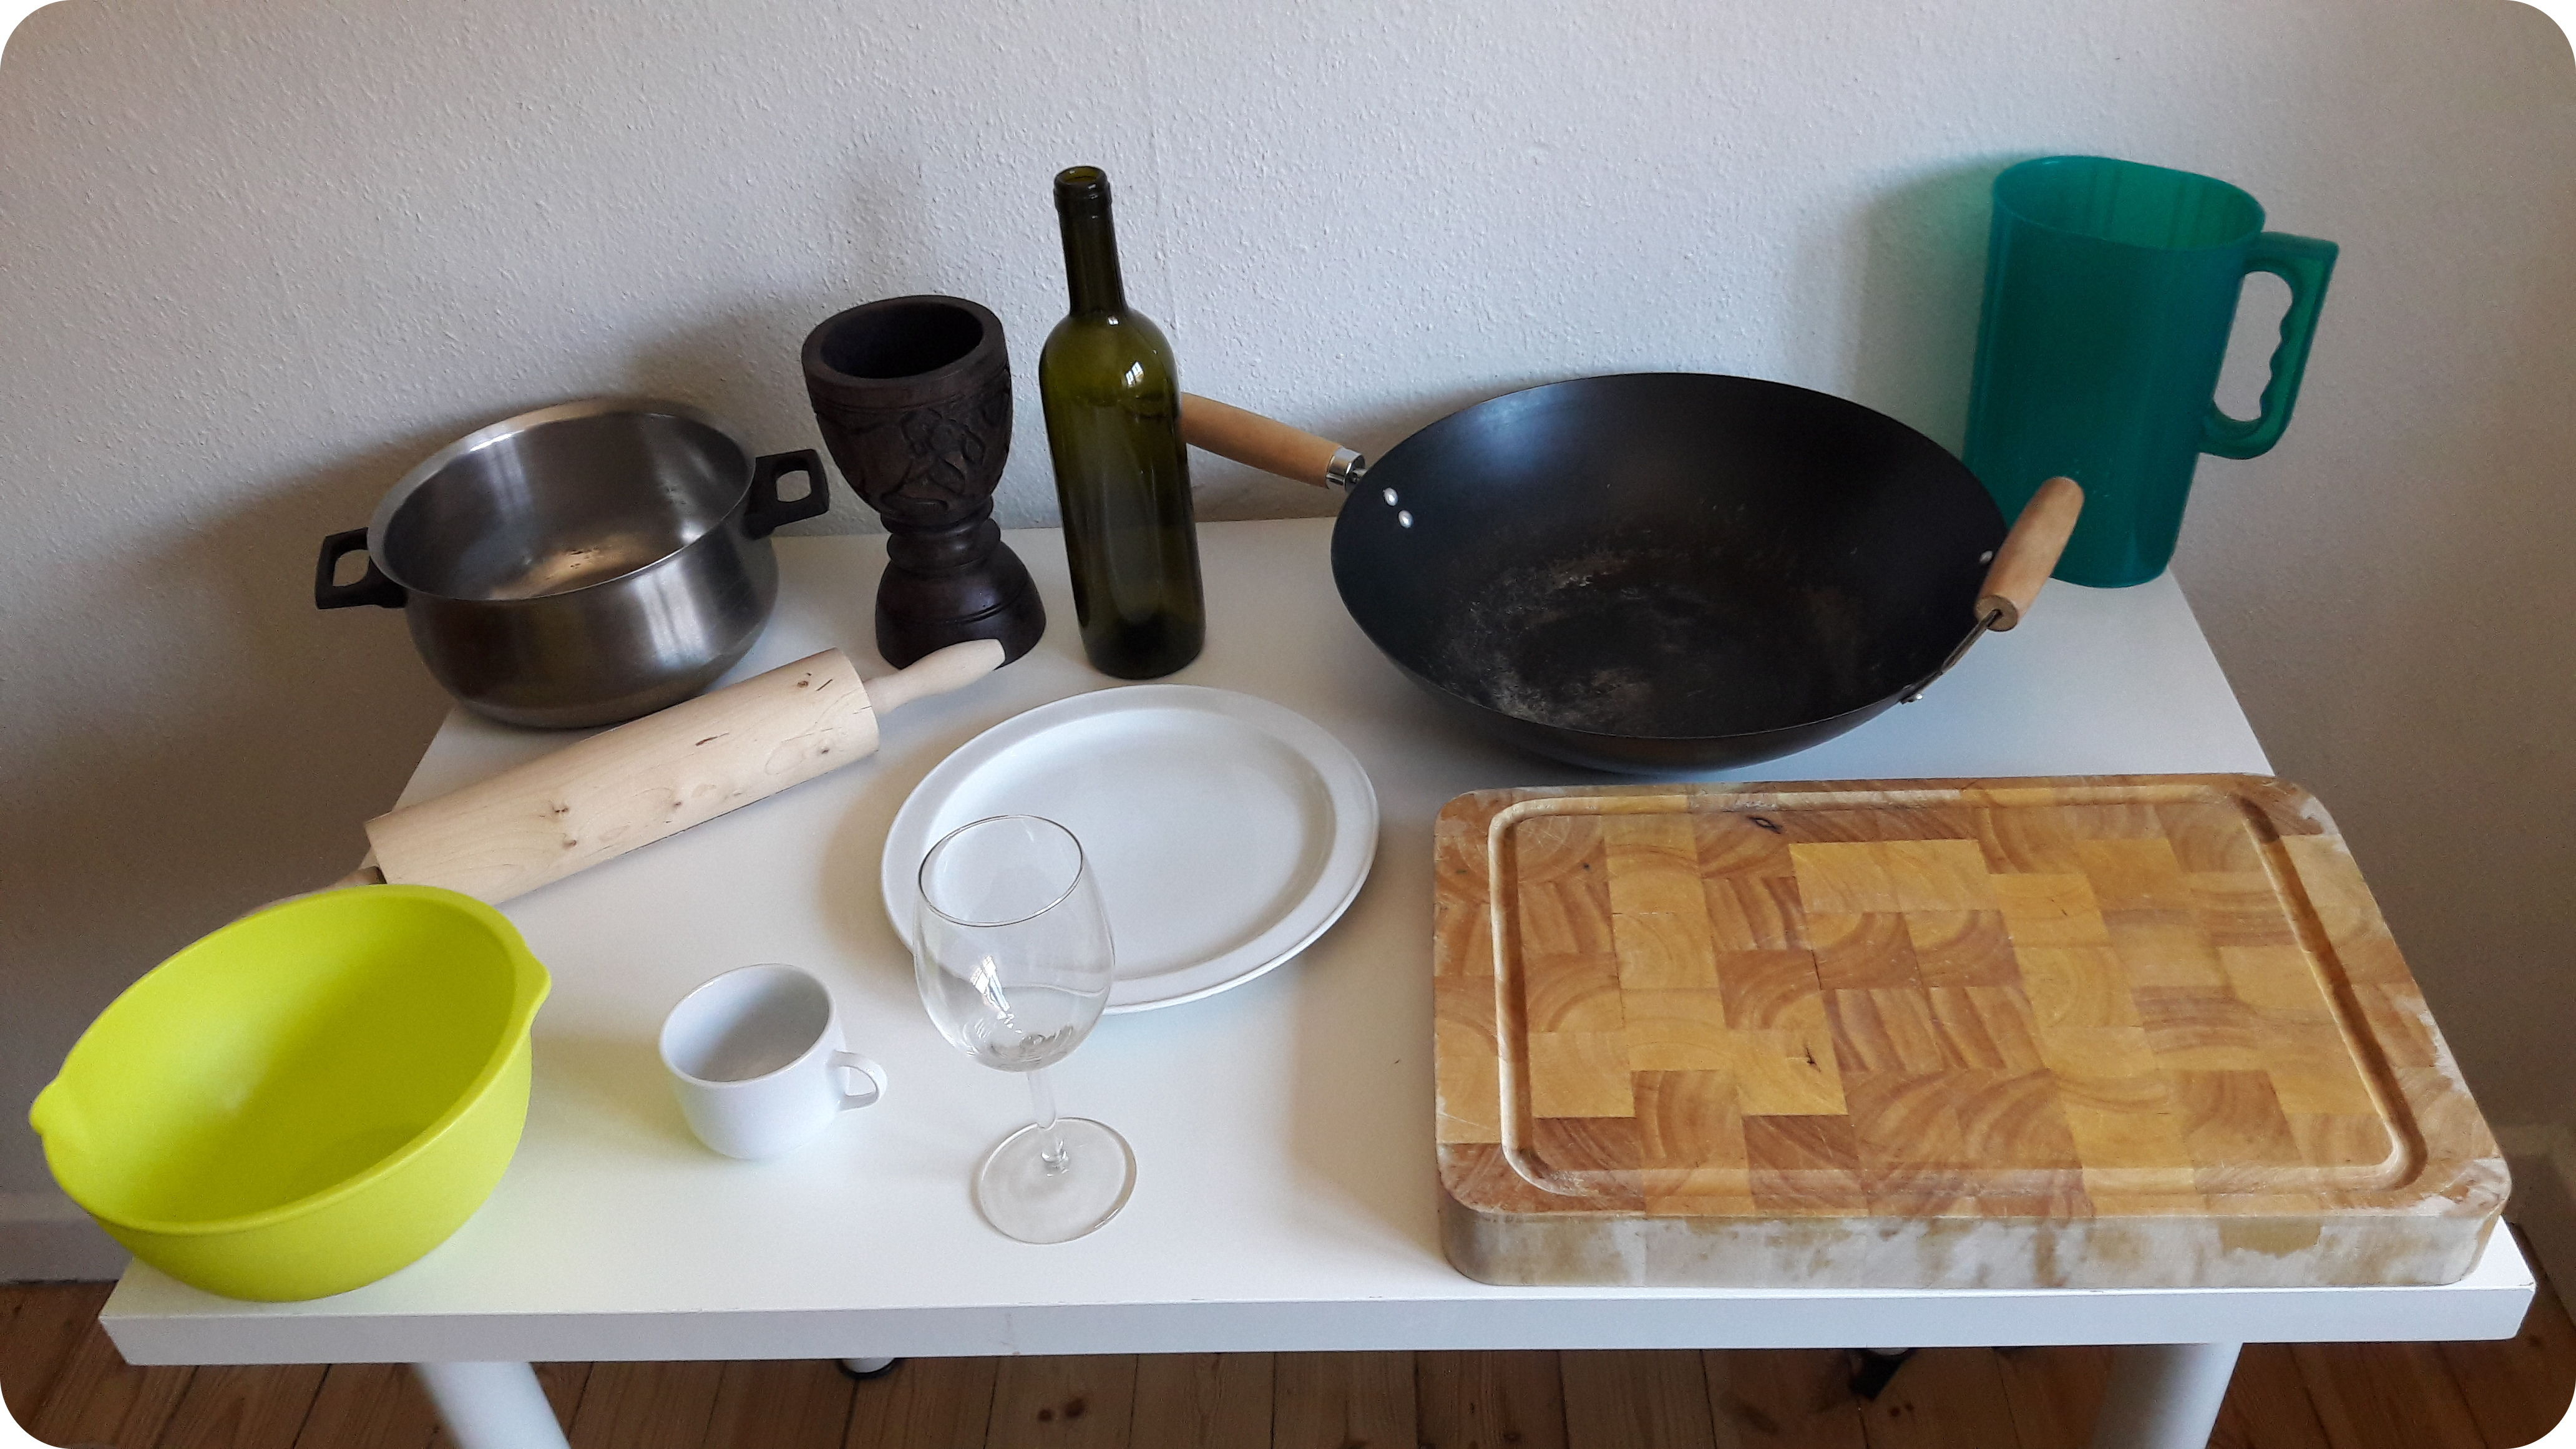
\includegraphics[width=\textwidth]{realobjects_r.jpg}
        \caption{Real objects.}
        \label{fig:real}
    \end{subfigure}
    ~ %add desired spacing between images, e. g. ~, \quad, \qquad, \hfill etc. 
      %(or a blank line to force the subfigure onto a new line)
    \begin{subfigure}[b]{0.8\textwidth}
        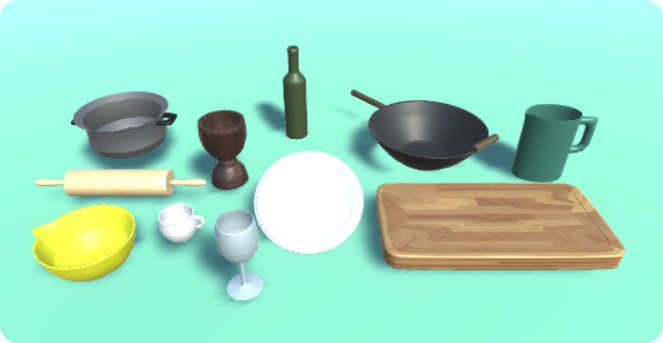
\includegraphics[width=\textwidth]{3dobjects_r.PNG}
        \caption{3D models of the objects.}
        \label{fig:models}
    \end{subfigure}
    \caption{The eleven objects used in the thesis.}\label{fig:objects}
\end{figure}

\section{Modal data}
The modes detector algorithm described in section \ref{sec:chuck} was used to extract the modal data - frequencies and their corresponding amplitudes - from the recordings. Figure \ref{fig:bottle_data} shows the data extracted for the wine bottle object. Each graph corresponds to one of the ``sound areas'' we have divide it into.


Although, theoretically, each object can be modeled using one vector of frequencies and multiple vectors of amplitude data (one for each different vertex) we can see in figure \ref{fig:bottle_data} that this does not happen in practice. There are multiple reasons why, with the most notable being the possible discrepancies of the data extracting algorithm. In addition, to include all the resonant frequencies of one object, instead of the ones with the strongest peaks per area, we would need a very big frequency vector. This would take up a lot of memory space, without improving significantly the result. However, other causes could be the environment noise, the difference in the force when hitting the object or the way it is hold when being hit, during the recordings.


\begin{figure}[H]
  \centering
    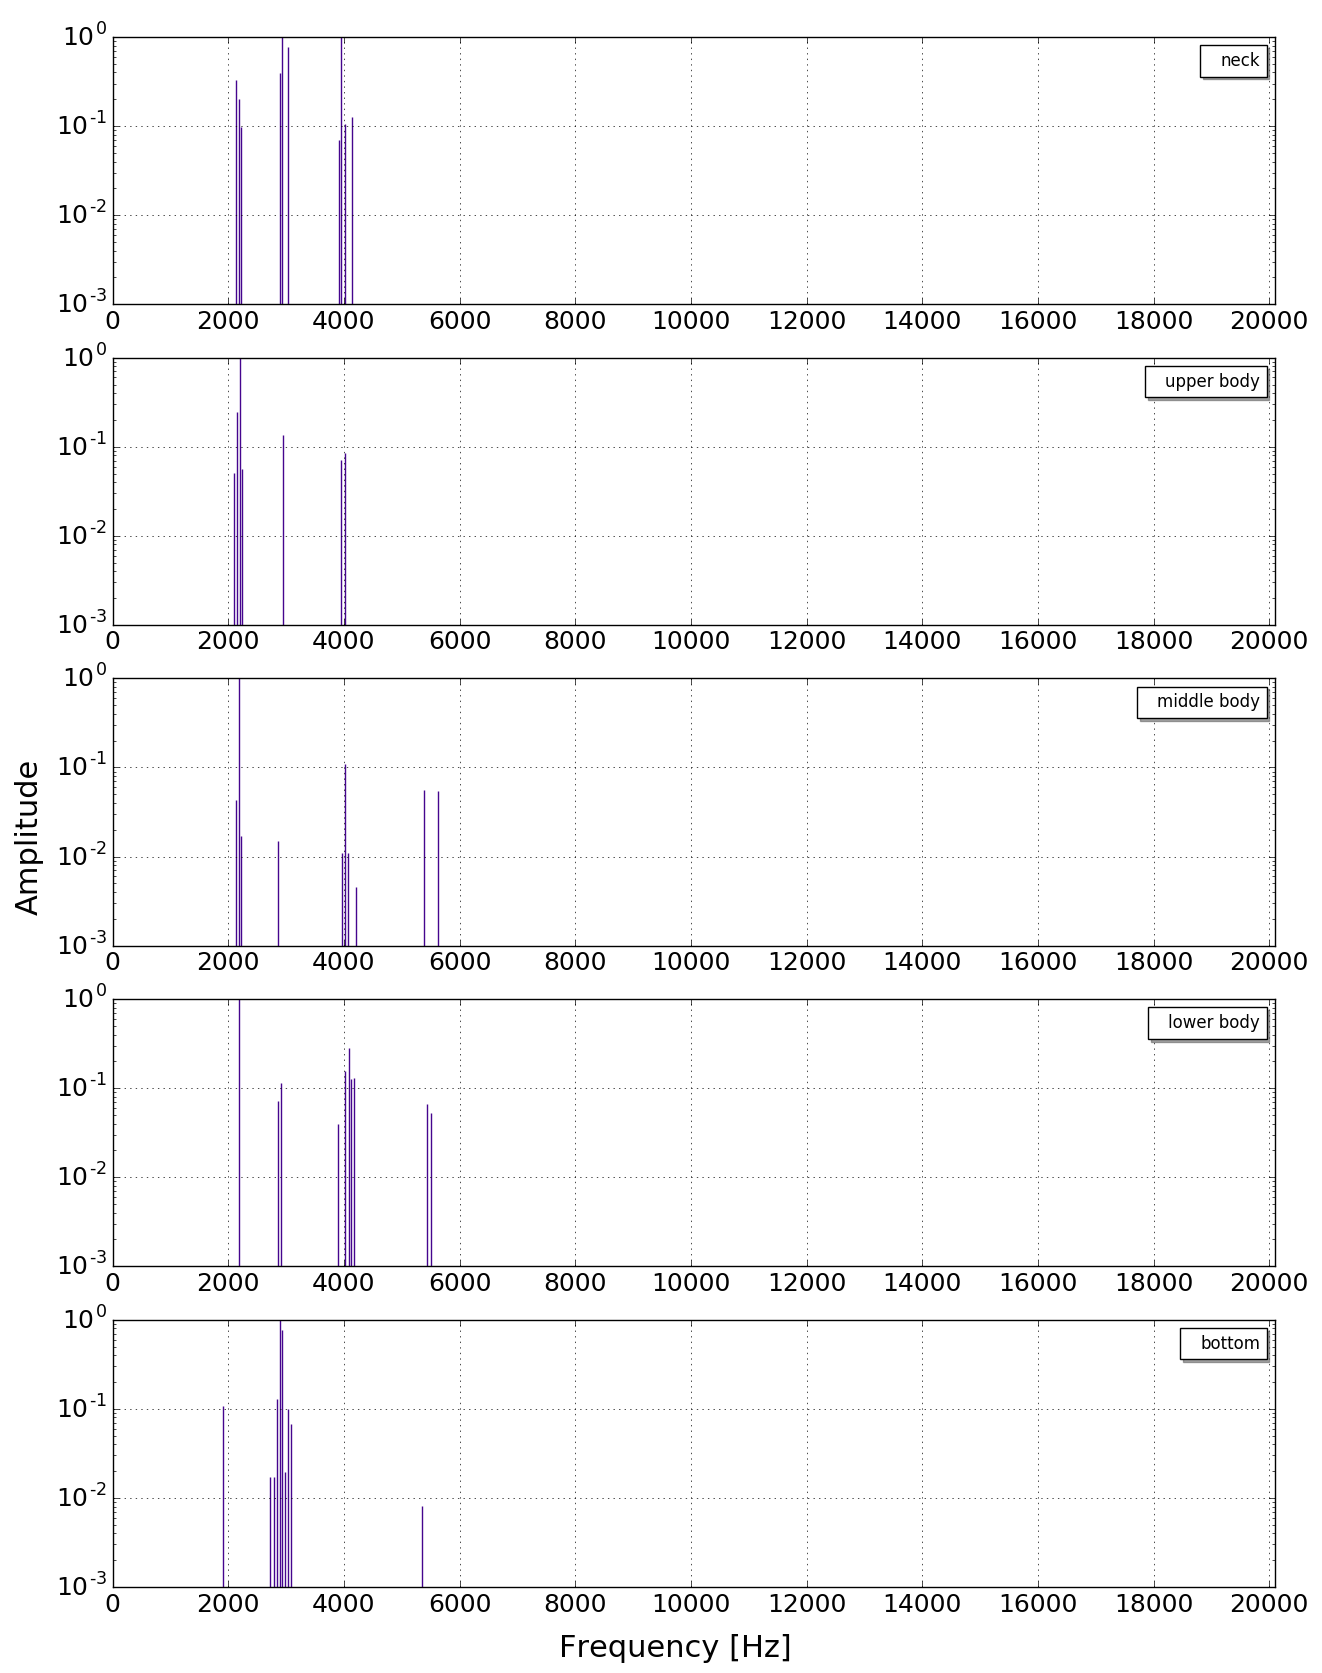
\includegraphics[width=0.9\textwidth]{winebottle.png}
      \caption{The frequencies and their corresponding peaks for each part of the wine bottle object.}\label{fig:bottle_data}
\end{figure}

Nevertheless, it is obvious that the fundamental frequencies are similar for each graph and lay just above 2000 Hz for the wine bottle.

\section{Sound Synthesis}\label{sec:synthesis_implem}

All synthetic sounds have been created in \gls{Pd} patches and are interpreted by Heavy which generates audio plugins and a C\# interface for Unity\textsuperscript{\textregistered}. This C\# script is attached to the GameObject in the scene so that the sound is processed within the game world.


A C\# script assigns to every one of the objects the modal parameters that were extracted in the analysis part (see section \ref{sec:chuck}). This is done independently of the synthesis methods used below.

Two different types of force models are considered as input to the synthesis patches. Impact forces that are used for sounds produced by a collision and constant contact forces, used for rolling and scratching sounds.

\subsection{Impact Sounds}\label{sec:impact_synth}
%\Todo{decribe the patch, describe the sound (starts low, goes to max ampl and then decays etc)}\\
%\Todo{Put spectrogram pictures of the sounds to describe them}
%
\subsubsection{Sinusoidal Additive Synthesis}\label{sec:sinusoidal_synth}

This section describes in depth how the \gls{Pd} patch corresponding to the sinusoidal additive synthesis of impact sounds works. The patch attempts to translate equation \ref{eq:modal_response} into the programming language of \gls{Pd}. Some of its terms are referenced in the following explanation.

First of all the frequencies and amplitudes matching the ten modes of the object are initialized. Therefore, these frequencies which we identified as $f_n$ in the equation \ref{eq:modal_response}, can be fed into the different oscillators. In \gls{Pd}, oscillators output a cosine wave which is equivalent to $cos(2 \pi f_nt)$ from the equation which suits our purpose perfectly.

\begin{figure}[H]
  \centering
    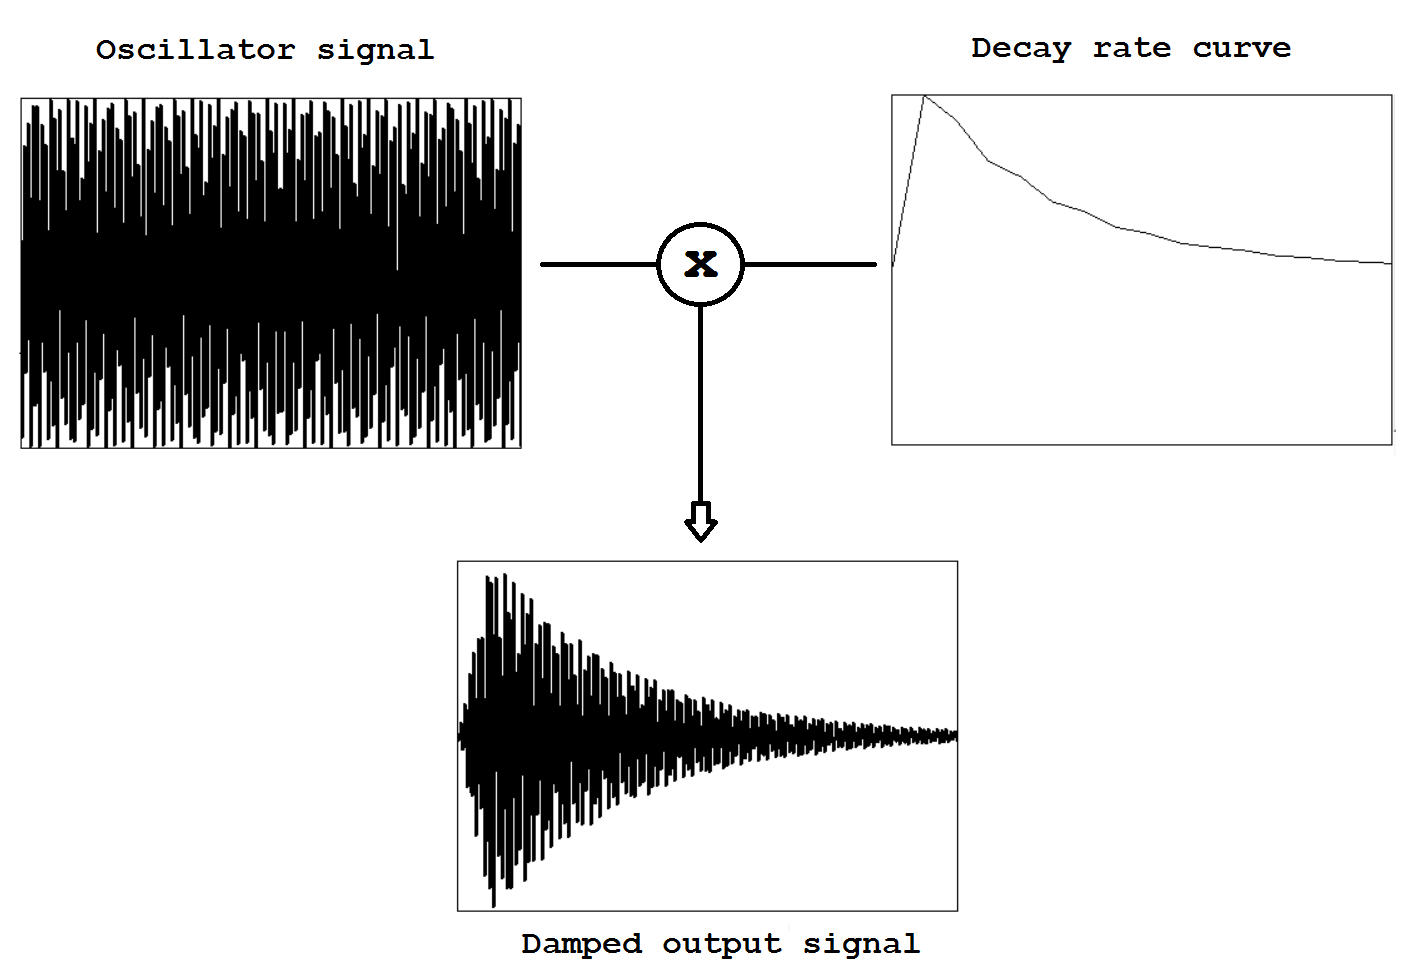
\includegraphics[width=0.7\textwidth]{dampedsignal.png}
      \caption{Diagram showing how the output partial is created from a 5000 Hz cosine wave and a decay rate curve with D = 0.005.}
      \label{fig:dampedsignal}
\end{figure}

The expression $e^{-d_n t}$ which corresponds to the damping of every mode $n$ is also translated into \gls{Pd}. Gaver, in \cite{gaver1993we}, states that for each partial the decay rates $d_n$ are controllable through a parameter $D$ which corresponds to a material and that a useful heuristic, that is used in the patch, is to have $d_n = 2 \pi f_nD$. By experimenting it was established that values of $D$ range from approximately 0.0002 for metal to about 0.05 for plastic sounds, with glass, ceramic and wood sounds in between. The higher the damping the higher the values. Then the damping is multiplied by the partial's initial amplitude $A_n$ to obtain an amplitude envelope that varies over time and which is multiplied by the oscillator's signal. The output is what is called a \textit{partial} which is illustrated in figure \ref{fig:dampedsignal}. 

The final sound is produced by adding together the ten partials. The resulting signal is multiplied by the magnitude of the impact. For this, the kinetic energy is calculated with Unity\textsuperscript{\textregistered}'s physics components (see section \ref{sec:coll_enter}). As described in \cite{farnell2010designing}, before sending the signal to the \gls{DAC}, it is passed through a clipper. This gives richer harmonics and produces brighter sounds the harder the impact is \cite{aramaki2009thinking}.

The patch produces an impact sound whenever the \textit{OnCollisionEnter} method from Unity\textsuperscript{\textregistered} is called. This is done when the collider, that has the script attached to it, has begun to touch another collider. When this happens we set the magnitude of the collision and then send an event to excite the patch. This is done by setting the value of $t$ in \ref{eq:modal_response} to zero which increases over time making the sound to decay.

\subsubsection{Filter-based Modal Synthesis}\label{sec:filter_synth}

This synthesis method is based on the utilization of a bank of ten bandpass filters. \gls{Pd}'s bandpass filters have three control inputs as seen in figure \ref{fig:pdbandpass}. The left inlet is the incoming audio signal, the middle one sets the center frequency and the right input sets the \gls{Q} factor value. The characteristics of these filters define the virtual object.

\begin{figure}[H]
  \centering
    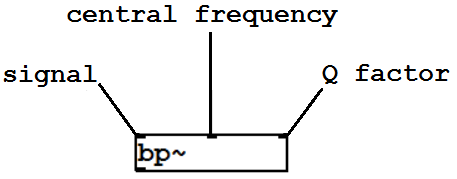
\includegraphics[width=0.5\textwidth]{bandpassfilter.png}
      \caption{Pd's bandpass filter with its three inlets}
      \label{fig:pdbandpass}
\end{figure} 

The same way it is done in the previous method, all ten frequencies and amplitudes of the object are initialized. Every frequency $f_n$ is sent into a bandpass filter as the center frequency. 

Every filter is characterized by its \gls{Q} factor which is directly related to the damping. The higher the value of \gls{Q}, the narrower the bandwidth and the less the resonator becomes damped. Thus, \gls{Q} determines the material of the impacted object \cite{gaver1993we}. By manipulating \gls{Q} different material sounds can be obtained. Through experimentation values of \gls{Q} that range from about 20 for plastic to 5000 for metal were found. 

To cause the object to sound an impulse signal that excites the filter is used. The amplitude of the signal is 1 at $t=0$ and 0 everywhere else, as represented in figure \ref{fig:impulse}. This impulse is multiplied by the value of the kinetic energy when the object impacts with a surface. 

\begin{figure}[H]
  \centering
    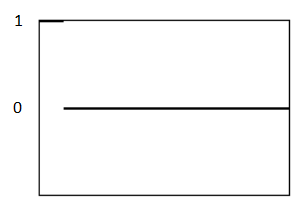
\includegraphics[width=0.5\textwidth]{impulse2.png}
      \caption{Impulse signal used to excite the bandpass filter.}
      \label{fig:impulse}
\end{figure} 

\gls{Pd} does not include a built-in impulse signal, thus it had to be constructed. The array shown in figure \ref{fig:impulse} was created to simulate a Dirac function which is commonly used to model impact events. For the purpose of this thesis the function is defined as

\begin{equation}\label{eq:dirac}
\delta (n) =  \begin{Bmatrix}
1$ , $n = 0
\\ 
0$ , $n > 0
\end{Bmatrix}
\end{equation}


with $n$ being the sample index and $\delta$ the Dirac function. The values of this array are read as the input signal. Since the lowest amount of time calculated by \gls{Pd} proved to be 2 milliseconds, it was not possible to read a small fragment of the input signal. Therefore, the impulse array was set to size 441, which is the number of samples per 10 milliseconds an the input array was read in a duration of the sample rate.

The output signal of each of the ten filters is multiplied by the corresponding amplitude $A_n$ of the mode. All ten resulting signals are added together. The signal is sent through a clipper as we did in the previous synthesis method.

\subsection{Scratching Sounds}\label{sec:scratching_synth}

\begin{figure}[H]
  \centering
    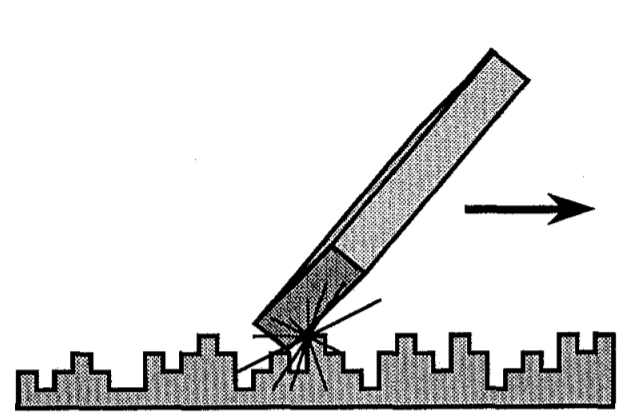
\includegraphics[width=0.5\textwidth]{microcollisions.png}
      \caption{Scratching involves a multitude of micro-collisions against a contact area. Picture from \cite{gaver1993we}}
      \label{fig:microcollisions}
\end{figure}

The sound produced by an object that is scraped across a rough surface can be assimilated to a succession of multiple impacts in a short time according to \cite{gaver1993we}. Additionally, the aforementioned paper shows that the resonant modes present in the spectrum of a struck object, are the same as when the object is scrapped. The same modal parameters can then be used as in the impact methods described here above.

To produce scratching sounds a similar technique to \cite{gaver1993we} and \\ \cite{van2001foleyautomatic} who propose the use of filters is followed. The filter-based modal synthesis method is therefore chosen to model the resonator as seen in the previous section. The difference lies in the signal that excites the model. This is implemented by generating a noise impulse waveform, as seen in figure \ref{fig:scratchingimpulse}, that passes through the bandpass filters. This waveform is created by having a simple impulse signal that is scaled relative to the velocity and material of the object and then multiplied by a white noise signal. From a heuristic approach it was deduced that the higher the velocity and the \gls{Q}, the higher the gain of the scratching sound. The length of the excitation signal depends on the time it took Unity\textsuperscript{\textregistered} to complete the last frame. The scraping sound is triggered in Unity\textsuperscript{\textregistered}'s OnCollisionStay method when the object's collider is touching another one and with the condition that the angular velocity of the object is beneath a threshold. The angular velocity specifies the rotational motion of a rigid body \cite{sears1964university}. This condition is therefore added to differentiate between sliding and rolling.

\begin{figure}[H]
  \centering
    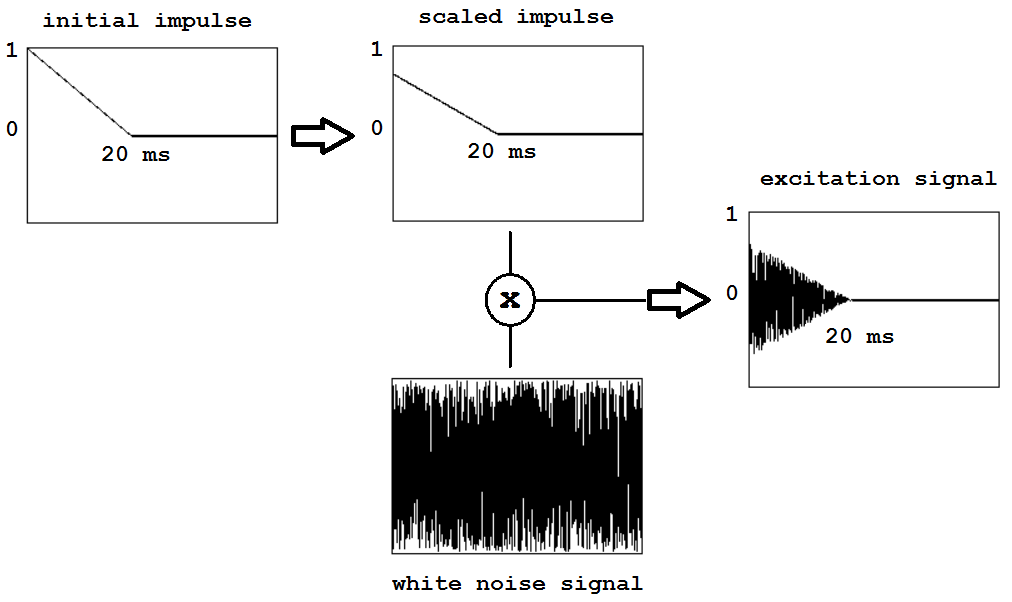
\includegraphics[width=0.9\textwidth]{scratchingexcitation.png}
      \caption{Diagram showing the process to get the excitation signal of the resonator to produce scratching sounds.}
      \label{fig:scratchingimpulse}
\end{figure} 

The authors who's approach is followed state that the center frequencies of the band-pass filters are scaled with respect to the contact velocity. The higher the velocity, the more the proportion of high-frequency energy increases. To recreate this effect the incoming filter frequencies are scaled depending on the velocity of the sliding object.

\subsection{Rolling Sounds}\label{sec:rolling_synth}

As well as scratching sounds, rolling sounds are produced by the irregularities of the surfaces in contact \cite{van2001foleyautomatic}, namely the rolling object's surface and the ground. This study therefore focuses on two models inspired by \cite{farnell2010designing}: a series of repetitive impulses that correspond to the surface profile of the rolling object and the irregular bumping sounds due to the uneven ground.

First the attention is directed to the sounds produced by the object's surface irregularities. For simplification a regular octagon that has received an impulsive force is used and therefore rolls along a plane. Every time one of the vertices impacts the ground, energy is lost to heat and sound. Thus, as the octagon rolls, a pattern of eight impulses is created for every rotation as seen on figure \ref{fig:rolling}. To create these impact sounds the filter-based synthesis method is applied. The filters are excited by a succession of eight impulses of different amplitudes as no real object has a perfect geometry. The outcome results in a pattern of quasi-periodic audio cues distributed differently over time depending on the speed of the rolling object. See figure \ref{fig:rolling}. \cite{houben1999auditory} and \cite{rath2003expressive} suggest that this periodicity which originates from the asymmetry of the object, enables listeners to distinguish between sliding and rolling sounds.


\begin{figure}[H]
  \centering
    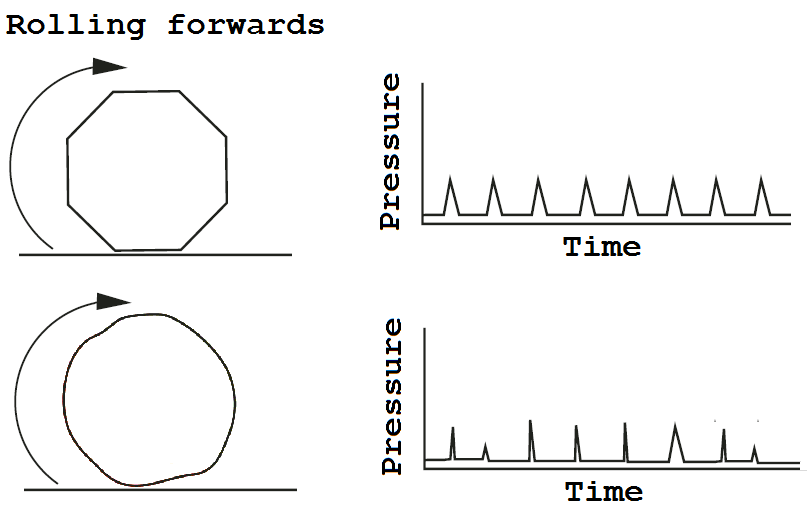
\includegraphics[width=0.7\textwidth]{rolling.png}
      \caption{An octagon and a real spherical object pressure levels over time as they roll.}
      \label{fig:rolling}
\end{figure} 

Let us dive into the actual implementation of the latterly described model. It was previously mentioned that the amplitude of the impulse signals used to excite the resonator are different. With a heuristic approach, a sequence of eight multipliers that correspond to the prominence of the bumps along the object's surface contour is chosen. Additionally, a parameter that determines the object's surface roughness has been incorporated. This parameter, which can be adjusted by the user, scales the values of the eight multipliers. The lower the value of the parameter the smoother the object's surface. In other terms, the smoother the object's surface, the smaller and more homogeneous the amplitude of the impulses are. The amplitudes of the impulses for different roughness degrees can be compared in figure  \ref{fig:roughnessgraph}.

\begin{figure}[H]
  \centering
    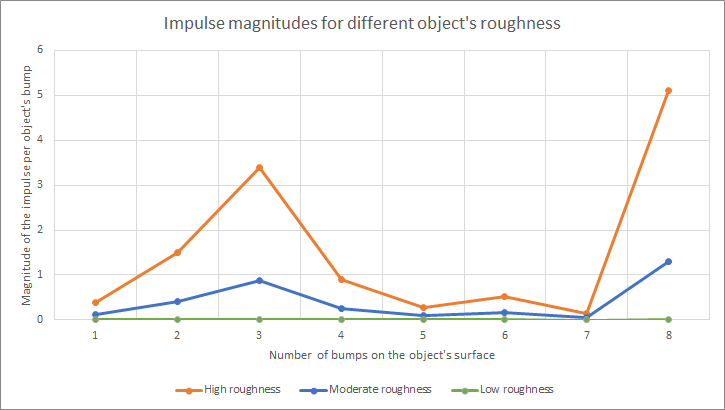
\includegraphics[width=\textwidth]{roughnessgraph.png}
      \caption{Graph showing the amplitude of the impulses for every bump on the object's surface for three values of the roughness parameter.}
      \label{fig:roughnessgraph}
\end{figure} 

We now look into the sounds produced due to the irregularity of the ground. As pointed out in \cite{van2001foleyautomatic}, even a smooth ball rolling on a rough surface produces sound. This paper and \cite{rath2003expressive} indicate that this is due to the small constant collisions of the ball with the surface's asperities. The bigger the ball, the less the surface details are``felt''. In our implementation the surface's irregularities are considered to be very small compared to the radius of the rolling object. See figure \ref{fig:rollingdoel}. This suggests that our model for uneven ground is similar to our previously explained scratching model as \cite{van2001foleyautomatic} proposes. The difference is that the gain of the output signal is lower for the rolling as rolling friction forces are considered to be smaller compared to scratching friction \cite{mehtas}.

\begin{figure}[H]
  \centering
    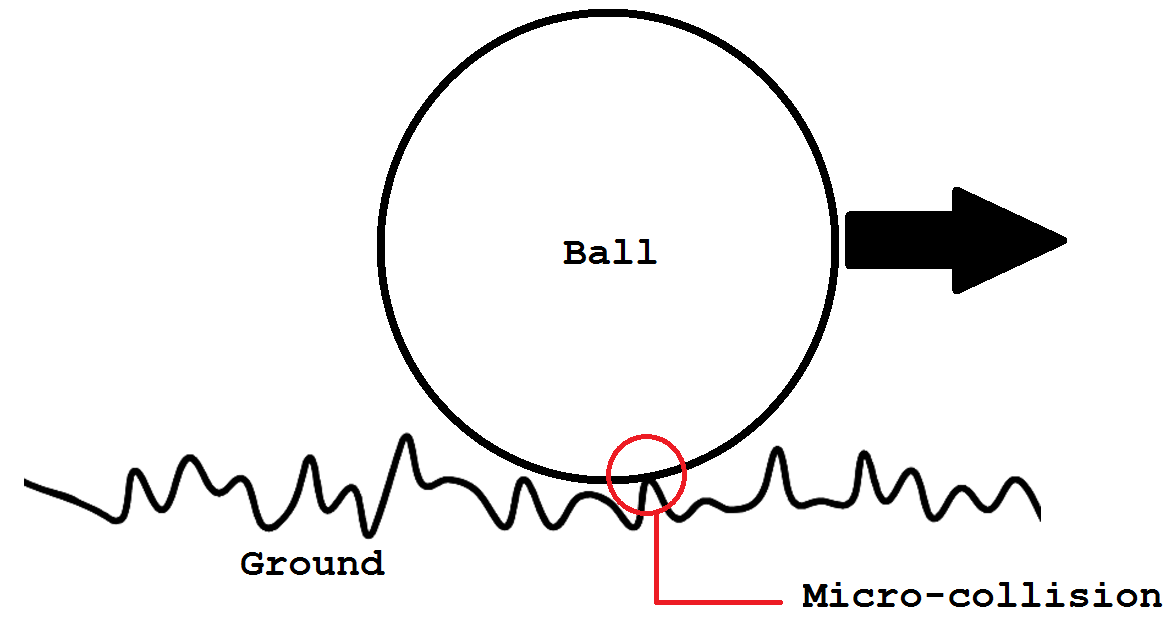
\includegraphics[width=0.6\textwidth]{rollingdoel.png}
      \caption{A smooth ball rolling over an small ground irregularities.}
      \label{fig:rollingdoel}
\end{figure} 



\section{User Interface}\label{sec:UI}
This section describes the \gls{UI} of the tool, where designers are able to tweak parameters and choose the sound they prefer for every object. The \gls{UI} is made inside Unity\textsuperscript{\textregistered}, by programming a custom inspector. \textit{Inspector} in Unity\textsuperscript{\textregistered} is a window that shows up inside the platform, after selecting an object, a file, etc. and it displays all information relevant to it. A custom \textit{GUISkin} is also used, which is a set of settings about the \gls{GUI}. 

When the designer wants to insert a new object with the audio implemented, he can either use one of the pre-made prefabs that have been created (which correspond to the modeled kitchen objects) or assign the procedural audio component on a Unity\textsuperscript{\textregistered} game object of his choice. In the second case, he only has to select this game object and then from the Unity\textsuperscript{\textregistered} menu bar he can select one of the two available methods described above, as seen in figure \ref{fig:menu_item}.

\begin{figure}[H]
  \centering
    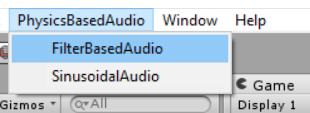
\includegraphics[width=0.5\textwidth]{menuItem.png}
      \caption{Designer can assign the audio manager from the menu bar.}
      \label{fig:menu_item}
\end{figure}

There are a number of components that are necessary for a game object. The ``Rigidbody'' which gives physics characteristics, the ``Audio Source'' that activates the sound, the synthesis plugin that generates  procedural audio, the ``Modal Data Script'' that assigns the correct modal data to the object and the ``Audio Manager Script'' which controls the audio events. An example of the whole Unity\textsuperscript{\textregistered} inspector of a modal object can be seen in figure \ref{fig:audio_insp}.

Since each set of modal data is related to one specific object, the tool is restricted to the objects available up to this time. Therefore, the designer has to assign a ``tag'' of one of the eleven objects available on the tool (cooking pot, cup, cutting board, jug, mortar, bowl, plate, rolling pin, wine bottle, wine glass or wok), if he uses his own objects. However, it is possible for everyone to contribute with new objects to the tool, by following the guide on appendix \ref{ap:guide}.

Figure \ref{fig:custom_insp} shows the three parameter sliders, available to designers for adjusting the audio. They are the same for both of the synthesis methods  used in this thesis (figures \ref{fig:FB}, \ref{fig:sin}). The first slider is the material selection. Although each object used in this thesis has a distinct type of material, designers are able to assign to them another material of the five available choices (plastic, wood, ceramic, glass, metal), or even a blend of two of them. The second slider, concerning the size of the object, can be used when the designer wants to introduce a smaller or bigger object than the default ones, or even when he prefers the sound to be more high or low pitched. The last slider adjusts the roughness of the object's surface. By tweaking this, designers are able to chose surfaces of the objects to be smoother of rougher than the default ones. Changing this parameters is perceived when the object is rolling. Below there is an extended description of the sliders.

\begin{figure}[H]
    \centering
    \begin{subfigure}[b]{0.45\textwidth}
        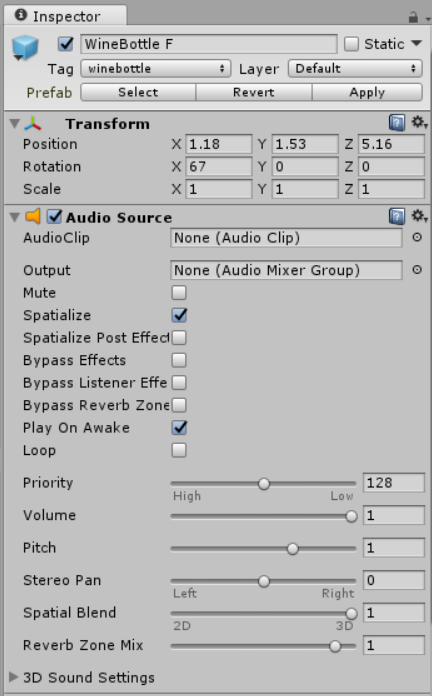
\includegraphics[width=\textwidth]{inspector1.PNG}
        %\caption{Upper part}
        \label{fig:FB}
    \end{subfigure}
    \vspace{-0.6cm}%
      
\hspace{-4pt}\begin{subfigure}[b]{0.45\textwidth}
        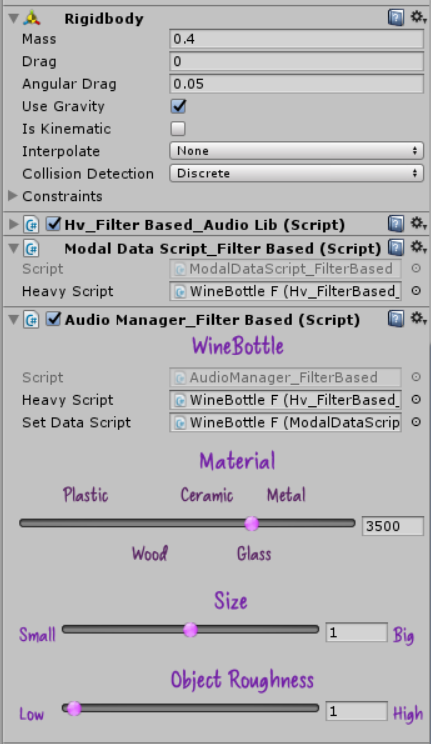
\includegraphics[width=\textwidth]{inspector2.PNG}
        %\caption{Lower part}
        \label{fig:sin}
    \end{subfigure}
    \caption{An example inspector of a game object inside Unity\textsuperscript{\textregistered} platform.}\label{fig:audio_insp}
\end{figure}


\begin{figure}[H]
    \centering
    \begin{subfigure}[b]{0.45\textwidth}
        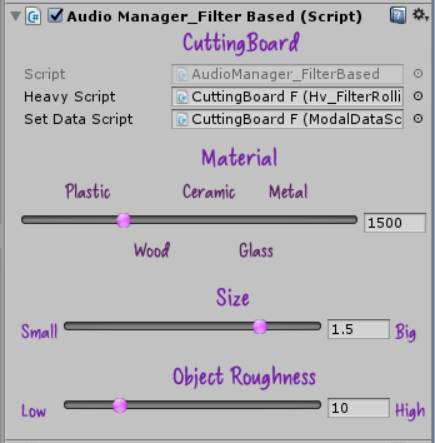
\includegraphics[width=\textwidth]{audio_managerF_inspector.PNG}
        \caption{Inspector of the filter-based modal synthesis method.}
        \label{fig:FB}
    \end{subfigure}
    ~ %add desired spacing between images, e. g. ~, \quad, \qquad, \hfill etc. 
      %(or a blank line to force the subfigure onto a new line)
    \begin{subfigure}[b]{0.45\textwidth}
        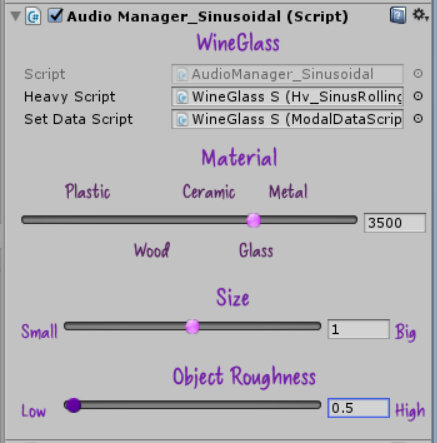
\includegraphics[width=\textwidth]{audio_managerS_inspector.PNG}
        \caption{Inspector of the sinusoidal additive synthesis method.}
        \label{fig:sin}
    \end{subfigure}
    \caption{The custom inspector inside Unity\textsuperscript{\textregistered} platform with the parameters available to designers.}\label{fig:custom_insp}
\end{figure}

\subsection{Changing the Material}
Different materials can be assigned to the objects used in this tool. The designer is able to choose between \textit{Plastic, Wood, Ceramic, Glass} and \textit{Metal} by adjusting the corresponding slider on the interface (see figure \ref{fig:custom_insp}). 

Metallic or glass sounds are more ``ringy'' than wooden or plastic ones that are more ``thud''. We achieve those sounds by changing the \gls{Q} factor of the band-pass filters used in the \GLS{Pd} patch. The \gls{Q} indicates the power loss in the filter. The higher the \gls{Q} the less power is lost, so the resonator vibrates longer as explained in equation \ref{eq:Qfactor} \cite{bib:Q}.

\begin{equation}\label{eq:Qfactor}
Q=2\pi \frac{\mbox{maximum energy stored}}{\mbox{total energy lost per cycle at resonance}}
\end{equation}

Using trial and error methods, an approximate value of the \gls{Q} for each material is chosen and used as the default value in the tool. Those values are shown in the table \ref{tab:default_Q}.

\begin{table}[H]
	\centering
    \begin{tabular}{ l  c }
    \toprule
    \textbf{Material} & \textbf{Average Q-factor} \\
    \toprule 
    Plastic & 1000 \\ 
    Wood & 1500 \\ 
    Ceramic & 3000 \\ 
    Glass & 3500 \\ 
    Metal & 4000 \\
    \bottomrule
    \end{tabular}
    \caption{Default values of \gls{Q} factor for each material in the tool.}
    \label{tab:default_Q}
\end{table} 

\subsection{Changing the Size}
In an application, the same object can appear in different sizes. It is known that under the same excitation, the smaller the size of an object, the more high-pitched sounds it will produce \cite{gaver1993world}. Hence, a slider is implemented for the designer to choose the best sound that corresponds to the size of the object. It is to note that the middle position of the slider (\textit{size: 1}) corresponds to the real object used for the data extraction. The slider allows to size the object from a tenth of its original size to the double, to keep the frequencies in the audible range.

\subsection{Changing the Surface Roughness}
Another setting that the sound designer is able to tweak is the object's roughness. This parameter determines how irregular or ``bumpy'' the surface of the object is, therefore it affects rolling sounds as seen in section \ref{sec:rolling_synth}. By increasing the roughness of the object with the slider the more noticeable the impacts caused by the micro-collision are. When the slider is set to the lowest roughness coefficient, this corresponds to a perfectly smooth surface which ideally will not produce any sound.


\section{Unity\textsuperscript{\textregistered} Scripts}
Heavy \cite{bib:heavy} compiler was used to convert the \gls{Pd} patches described above into Unity\textsuperscript{\textregistered} compatible C\# code. However, several other scripts were implemented for the following actions: 
\begin{inparaenum}[1)]
\item Identify the type of the object and assign the corresponding modal data
\item Calculate the scale of the object if any
\item Detect which point of the object collided and assign the corresponding modal data
\item Calculate the impact force
\item Calculate distance traveled when rolling
\item Start an impact, rolling or scratching sound 
\end{inparaenum}.   

\subsection{Scaling}
As mentioned above, impact sounds are more high-pitched when an object is scaled down and \textit{vice versa}. To achieve a realistic scaling when the designer uses the built-in scaling feature of Unity\textsuperscript{\textregistered}, the tool calculates the size of the game object on start. More specifically, a \textit{scaling average (avgScale)} is calculated, taking into account all three dimensions:

\begin{lstlisting}[language=C]
avgScale = local scale of x dimension + local scale of y dimension + local scale of z dimension / 3
\end{lstlisting}

This average is used as an adder to the \textit{size parameter} described above. To avoid distortion in sound and to stay within the audible sound frequencies, we set a limit of adding $8.5$, a number found heuristically. This is considered to be a good choice because Unity\textsuperscript{\textregistered} uses \textit{meter} as the default unit and since everyday objects are focused on, it is rare for someone to use objects more than $8.5$ times its original size.

Then, the tool checks whether a scale-up or a scale-down was executed. In the first case, a normalization to $1/10$th of the average scale value is performed. The resulting scaling is applied to the size slider value and then to the pitch multiplier which we use to re-set the modal frequencies. To be more precise, instead of applying the actual pitch multiplier added with the average scaling, we subtracted from 2 and then we use it ($2-temp$ on the code below). This happens because we reversed the size slider. More specifically, the multiplier directly applied to the frequencies, increases them when it is bigger and decreases them when it is smaller. However, for convenient reasons, we wanted it to be the bigger the multiplier, the bigger the object and reverse. Since $2$ is the biggest value, we normalized it to be the smallest one.

In the second case, we subtract the value from the pitch multiplier. We do not need to normalize the average scaling value, because it is already between $0$ and $1$. Afterwards, we follow the same procedure as above, with one difference; instead of subtracting the new pitch multiplier from $2$ we add it to $1$. This happens because now the biggest value of the size slider is $1$ -since above this it counts as a scale-up- and we still want the reversed value for the slider, so we subtract the subtracted value, making it a plus ($+$). If no scaling took place nothing happens.

\begin{lstlisting}[language=C]
IF average scale > 1 (scale-up) THEN
    DIVIDE average scale by 10 to normalize
    ADD the normalized value to the pitch multiplier
    STORE new pitch multiplier to the size slider
    CALL SetTheFreqs to re-set the modal frequencies
ELSE IF average scale < 1 (scale-down) THEN
    SUBTRACT average scale from the pitch multiplier
    STORE new pitch multiplier to the size slider
    CALL SetTheFreqs to re-set the modal frequencies
END IF
\end{lstlisting}



\subsection{Excitation of Impact Sounds}\label{sec:coll_enter}
This is were the tool detects a collision of an object with something else. The collision could be either with the ground, another object from the tool or just an object in the scene. The program identifies when two Unity\textsuperscript{\textregistered} collider components attached to two different objects touch each other.

\paragraph{OnCollisionEnter function\\}

\textit{OnCollisionEnter} \cite{bib:unity_doc} is a Unity\textsuperscript{\textregistered}'s built-in function, which gets called when an object enters a collision.

The first thing that happens when a collision takes place, is to identify what kind of object is the one that collided with something, and which part of the object collided. Hence, a function is called which detects the type of the object using the tag manager. The tag manager holds all available tags. Tags are used to group similar game objects and make them retrievable from scripts. After the type of object is identified, the object perimeter variable (used for rolling sounds) is assigned to its corresponding value. Then, the modal data (frequencies and amplitudes) that correspond to this type of object are assigned to the variable used from the algorithm.

Moreover, the algorithm calculates the kinetic energy of the whole collision, using the equation \ref{eq:kinetic_energy} \cite{crowell2003conservation}: 

\begin{equation}\label{eq:kinetic_energy}
K = \frac{1}{2} m u^2,
\end{equation}

\noindent where $m$ is the mass of the object under test and $u$ the magnitude of the relative velocity between the two colliding objects. In Unity\textsuperscript{\textregistered} the latter can be calculated using the command: \textit{Collision.relativeVelocity.magnitude} \cite{bib:unity_doc}. The kinetic energy corresponds to the collision force magnitude and we use it to determine the output sound amplitude depending on whether the collision was strong or weak.

Another parameter that the algorithm takes into account is whether an object collides with another modal object or not. By modal object we mean the object that our tool provides that comes with modal synthesis sounds. In case a collision with another modal object occurs, the collision force magnitude is modified depending on the materials of both colliding objects. More specifically, an average between the two normalized quality factor values is calculated, it is then multiplied by the collision force magnitude and added to the initial collision force magnitude. This is done because the material of an object and thus its ``hardness'' (as seen in \cite{giordano2003material}) affects the ``loudness'' of the produced sound as shown through experimentation in \cite{freed1990auditory}. As a result when two hard materials like glass or metal collide with each other, they produce a much more intense sound than when a hard material collides with a softer one like plastic or wood.  

\begin{equation}
new\ CFM = CFM + CFM*\left( \frac{\frac{Qfactor_1}{5000} + \frac{Qfactor_2}{5000}}{2} \right)
\end{equation} 
\noindent where $CFM:$ the Collision Force Magnitude.

\Todo{see if it is necessary to describe the 3 different DACs here or just in the patch }

\subsection{Excitation of Rolling and Scratching Sounds}
\paragraph{OnCollisionStay function\\}

Unity\textsuperscript{\textregistered}'s built-in function \textit{OnCollisionStay} \cite{bib:unity_doc} is called once per frame as long as two rigidbodies are touching. Inside this function the program decides whether rolling or scratching takes place and calculates the corresponding velocity which stops the sound when it goes down to zero. The magnitude of this velocity is computed using the velocity vector of the object's \textit{Rigidbody} (\textit{rigibody.velocity.magnitude}). Unity\textsuperscript{\textregistered}'s rigidbody is ``the way of controlling an object's position through physics simulation'' as noted in Unity\textsuperscript{\textregistered}'s documentation API \cite{bib:unity_doc}.

The decision of whether an object is rolling or sliding along a surface is made using the angular velocity ($\omega = \frac{angular\ displacement}{time}$). Unity\textsuperscript{\textregistered}'s rigidbody variable for angular velocity is a three dimensional vector, measured in radians per second \cite{bib:unity_doc}. The magnitude of it is calculated from the equation \ref{eq:angVelMagn}
\begin{equation}\label{eq:angVelMagn}
\omega_{magnitude} = \sqrt{\omega_x^2+\omega_y^2+\omega_z^2}
\end{equation}
where $\omega_x = \frac{\theta_x}{t}, \omega_y = \frac{\theta_y}{t}, \omega_z = \frac{\theta_z}{t}$ and $\theta_x, \theta_y, \theta_z$ the angular displacement of the $x, y, z$ axis respectively and $t$ the amount of time this displacement lasted. In Unity\textsuperscript{\textregistered} it is referred to as (\textit{rigidbody.angularVelocity.magnitude}) \cite{bib:unity_doc}. More specifically, when the angular velocity magnitude is over $1$, it means that the object is rolling, otherwise it is not and providing that the linear velocity is non-zero, it means that the object is sliding on the surface. \Todo{why 1 is the border? maybe because (0.0,0.0,0.0) angular velocity gives 0.smth in magnitude}

\Todo{add an Optimization section maybe?}







